\documentclass[12pt]{article}
\usepackage[margin=1in]{geometry}
\usepackage{arev}
\usepackage{pgfplots}
\usepackage[inline]{enumitem}
\usetikzlibrary{calc}
\pgfplotsset{compat=newest}

\begin{document}
\section*{Quiz}

For each slope field, sketch 3 particular solutions and select the corresponding

\begin{figure}[!hbt]
	\centering
	\newcommand\dd[2]{\frac{\mathrm{d}#1}{\mathrm{d}#2}}
	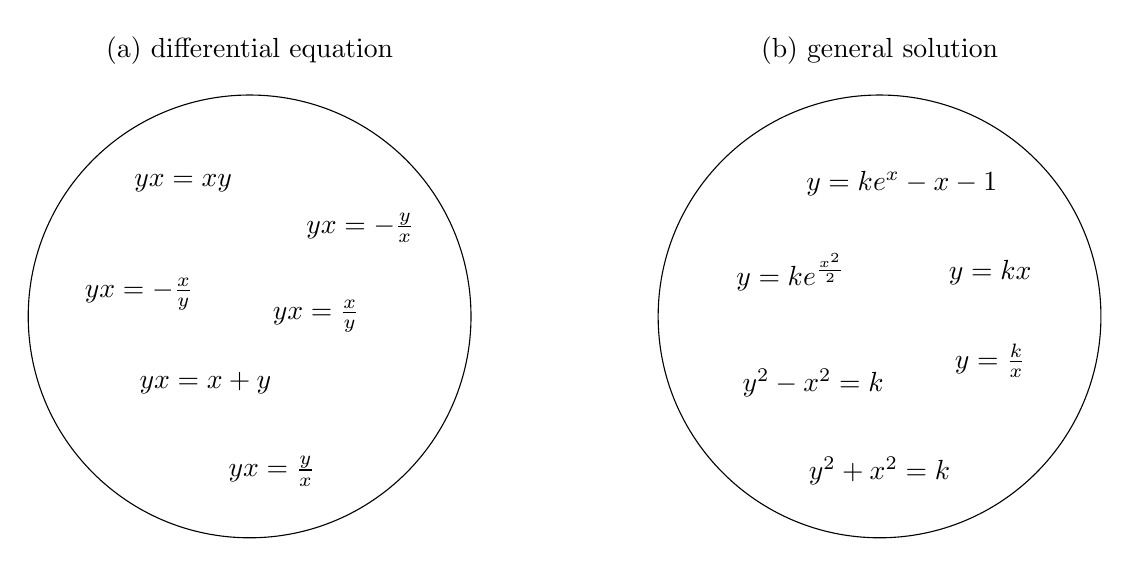
\begin{tikzpicture}
		\def\r{80pt}
		\coordinate (left) at (-4,0);
		\coordinate (right) at (4,0);
		\node at ($(left) + (0,1.2*\r)$) {(a) differential equation};
		\node at ($(right) + (0,1.2*\r)$) {(b) general solution};

		\draw (left) circle [radius=\r];
		\draw (right) circle [radius=\r];

		\node at ($(left) + (-0.2*\r,-0.3*\r)$) {$\dd{y}{x} = x+y$};
		\node at ($(left) + (-0.3*\r,0.6*\r)$) {$\dd{y}{x} = xy$};
		\node at ($(left) + (0.1*\r,-0.7*\r)$) {$\dd{y}{x} = \frac{y}{x}$};
		\node at ($(left) + (0.5*\r,0.4*\r)$) {$\dd{y}{x} = -\frac{y}{x}$};
		\node at ($(left) + (0.3*\r,0*\r)$) {$\dd{y}{x} = \frac{x}{y}$};
		\node at ($(left) + (-0.5*\r,0.1*\r)$) {$\dd{y}{x} = -\frac{x}{y}$};

		\node at ($(right) + (0.1*\r,0.6*\r)$) {$y=ke^x-x-1$};
		\node at ($(right) + (-0.4*\r,0.2*\r)$) {$y=ke^{\frac{x^2}{2}}$};
		\node at ($(right) + (0.5*\r,0.2*\r)$) {$y=kx$};
		\node at ($(right) + (0.5*\r,-0.2*\r)$) {$y=\frac{k}{x}$};
		\node at ($(right) + (-0.3*\r,-0.3*\r)$) {$y^2-x^2=k$};
		\node at ($(right) + (0*\r,-0.7*\r)$) {$y^2+x^2=k$};
	\end{tikzpicture}

	\vspace{1cm}

	\def\width{6.5cm} \def\height{6.5cm}
	% #1: differential equation
	\newcommand\slopefield[1]{
		\begin{tikzpicture}
		% domain and tick settings - note domain is square, change in axis options if needed
		\def\domainMin{-3}
		\def\domainMax{3}
		\pgfmathsetmacro\quiverScale{(\domainMax-\domainMin)/25}
		\begin{axis}[view = {0}{90}, % set camera to point towards x-y plane
			     domain=\domainMin:\domainMax,
			     xmin=\domainMin, xmax=\domainMax,
			     ymin=\domainMin, ymax=\domainMax,
			     ticks=none,
			     width=\width, height=\width,
			     axis equal image]
		    % draw axes
		    \draw[->,thick] (\domainMin,0)--(\domainMax,0);
		    \draw[->,thick] (0,\domainMin)--(0,\domainMax);
		    % plot unit length quivers with no head
		    \addplot3[black!60, quiver={u=1/(sqrt((#1)^2+1)), v=(#1)/(sqrt((#1)^2+1)), scale arrows=\quiverScale}, samples=16, forget plot] (x,y,0);
            \node[anchor=north west, fill=white] at (\domainMin, \domainMax) {\showFieldNumber.};
		\end{axis}
		\end{tikzpicture}
	}

    \newcounter{fieldNumber}
    \newcommand\showFieldNumber{\thefieldNumber\stepcounter{fieldNumber}}

	\slopefield{x+y} \hspace{\fill} \slopefield{x*y} \hspace{\fill} \slopefield{y/x} % top row

	\vspace{1cm}

	\slopefield{-y/x} \hspace{\fill} \slopefield{x/y} \hspace{\fill} \slopefield{-x/y} % bottom row
\end{figure}

\end{document}
